%% Journal of Biomedical Informatics (Elsevier) manuscript -- DRAFT (outline stage, 2026-08-06)
%%
%% Status: NOT submission-ready. Derived from manuscript/bmc_bioinformatics/manuscript.tex
%% (same claims, same numbers, same [STAGE] outline bullets) by porting from BMC's `bmcart`
%% class to Elsevier's `elsarticle` class and adapting to JBI's structure/format.
%%
%% Source of every claim below: results/EVALUATION_AUDIT.md (canonical, English),
%% results/PROTOCOLO_Y_CIFRAS_VIGENTES.md (Spanish quick-reference, same numbers). Every
%% number here must trace to an artifact under results/comparison/ -- do not hand-edit a
%% figure here without regenerating it from that artifact first.
%%
%% elsarticle.cls / elsarticle-num.bst in this directory are vendored, unmodified, from
%% Elsevier's official LaTeX author template (LPPL license, Copyright 2007-2026 Elsevier
%% Ltd -- see the header comment in elsarticle.cls). Identical copies already used
%% successfully in ~/Documents/iieg/papers/AIgave-fepaj2025/agave_paper/ on this machine.
%%
%% Format verification against JBI's live guide-for-authors (last attempted 2026-08-06):
%% that page (https://www.sciencedirect.com/journal/journal-of-biomedical-informatics/
%% publish/guide-for-authors) blocks automated fetches with a CAPTCHA -- tried direct
%% fetch, Wayback Machine, and a read-proxy, all blocked. Everything below is from
%% search-result fragments (some directly attributed to this page's indexed text, some
%% inferred from sibling Elsevier/ScienceDirect journals using the same author-guidelines
%% template) plus standard `elsarticle` convention.
%%
%% CONFIRMED (direct quoted fragments attributed to JBI's own guide page):
%%   - Structured abstract: Objective/Methods/Results/Conclusion, <=300 words.
%%   - Body structure: Introduction/Related Work/Methods/Results/Discussion/Conclusion,
%%     <=6000 words total.
%%   - `elsarticle-num` (numeric, Vancouver-style) citation/reference style.
%%   - Graphical abstract is OPTIONAL/encouraged, not mandatory (min 531x1328px, readable
%%     at 5x13cm, TIFF/EPS/PDF/MS Office) -- none included here by design.
%%   - Hybrid OA model, delayed access free route after 12 months (matches the earlier
%%     no-mandatory-fee research for this journal).
%% HIGH-CONFIDENCE INFERENCE (identical boilerplate text found verbatim on sibling
%% Elsevier/ScienceDirect journals in the same informatics family -- International
%% Journal of Medical Informatics, Computers in Biology and Medicine -- but not an
%% independently quoted fragment from JBI's own page specifically):
%%   - Highlights: 3-5 bullet points, <=85 characters each including spaces (applied
%%     below: 5 bullets, all <85 chars).
%%   - Keywords: "maximum of 6 keywords" (Elsevier's near-universal boilerplate across
%%     essentially all their journals on this template) -- trimmed from 8 to 6 below on
%%     this basis. STILL WORTH a final manual check before submission since this number
%%     was never seen quoted specifically for JBI, only inferred from the template.
%% NOT VERIFIED AT ALL: figure/table formatting rules beyond plain LaTeX
%% `tabular`/`tikz` (none applied; no JBI-specific rule surfaced in any search attempt).

\documentclass[review]{elsarticle}

\usepackage{cmap}
\usepackage{lmodern}
\usepackage{lineno}
\usepackage{array}
\usepackage{amsmath}
\usepackage{graphicx}
\usepackage{tikz}
\usetikzlibrary{arrows.meta, positioning}
\usepackage[colorlinks=true,citecolor=blue!60!black,linkcolor=black,urlcolor=blue!60!black]{hyperref}
\modulolinenumbers[5]

\journal{Journal of Biomedical Informatics}

\bibliographystyle{elsarticle-num}

\begin{document}

\begin{frontmatter}

\title{The Protocol, Not the Model: Evaluation Bias Inflates Link Prediction on
Biomedical Interaction Graphs}
%% STAGE: title. Two constraints, both decided explicitly -- do not drift either without
%% revisiting them.
%%   (1) No disease in the title (decision D1, 2026-07-17 -- see goal.md \S3.2 and
%%       results/PROTOCOLO_Y_CIFRAS_VIGENTES.md rule 5: the disease label is data
%%       provenance, never a claim). Keep the methods framing; do not let a later
%%       co-author drift it back toward a disease-discovery title.
%%   (2) Scope widened 2026-08-31, after the Results were reordered general-first. The
%%       old title said "Inflate microRNA--Target Link Prediction", which named the
%%       narrowest object in the paper: five of the six graphs carrying the headline
%%       claim are miRNA--DISEASE graphs, the two OGB benchmarks are drug--drug and
%%       protein--protein, and the 21-paper survey spans circRNA/lncRNA--disease,
%%       drug--target and gene--disease. "Biomedical interaction graphs" is the honest
%%       object; the trailing clause keeps microRNA discoverable and marks the primary
%%       case as one component, not the whole paper. Alternatives considered and
%%       rejected: leading with the audit ("An Audit of 22 Papers and a Six-Graph
%%       Replication"), leading with the number ("From 0.99 to 0.63"), and leading with
%%       the deliverable ("A Minimum Reporting Standard for..."). Dropped "Substantially"
%%       as redundant once the object is stated plainly.
%%   (3) Reworded 2026-09-07 (constraints (1) and (2) revisited and both still hold: no
%%       disease named, object still "biomedical interaction graphs"). The previous
%%       wording front-loaded both mechanisms and reached its verb at word seven, said
%%       "inflate link prediction" where what inflates is the MEASURED performance, and
%%       hung the case study on a trailing "with a..." clause. The new title is the
%%       paper's own Conclusion sentence -- the inflation is a property of the protocol,
%%       not of any one architecture or dataset. Two things were traded away knowingly:
%%       the two mechanisms are no longer named in the title (they open the Abstract's
%%       Methods and Results), and "microRNA" is no longer in the title -- indexing for
%%       it now rests on the keyword "microRNA--target prediction", the Abstract's first
%%       sentence, and the Highlights. Do not re-add a "with a microRNA--Target Case
%%       Study" tail to recover it; that was the clause this revision removed.

\author[aff1]{Ulises Moya S\'anchez\corref{cor}}
\ead{dr.ulisesmoya@gmail.com}
\cortext[cor]{Corresponding author.}
%% TODO: add remaining authors (advisor, any collaborators) with \author[aff...]{...},
%% repeating the block above (add \eaad{} only for the corresponding author). Order and
%% inclusion criteria are an authorship decision, not a technical one -- do not guess.

\address[aff1]{TODO -- institution/department, TODO city, TODO country}
%% TODO: fill in the real affiliation before submission.

\begin{abstract}
\textbf{Objective:} We audit whether Graph Neural Network (GNN) link-prediction evaluation practice inflates
reported performance, across ten cases spanning eight distinct graphs, to help
correct how link prediction is evaluated on biomedical interaction graphs.

\textbf{Methods:} The same topological heuristics and a graph transformer, trained
under a conventional evaluation protocol and one correcting transductive edge
leakage and popularity-biased negative sampling, were compared across ten cases spanning eight distinct
graphs: two Open Graph Benchmark (OGB) datasets, seven survey-paper datasets, and
our own graph (public single-cell RNA-seq data with miRDB v6.0 interactions). On our
own graph only, five further models (a homogeneous Graph Convolutional Network
(GCN), two ablations, a graph-free Multi-Layer Perceptron (MLP), and an untrained
control) and an unrelated cell-typing task with two graph-free controls were
tested under both protocols.

\textbf{Results:} Retraining one architecture under both protocols on six
graphs (ours and five from surveyed papers) lowers the Area Under the
Receiver Operating Characteristic curve (AUROC) from 0.879--0.992 to 0.618--0.641, a loss of 0.26--0.37 on each. For model-free heuristics (heuristics that use only graph topology), negative sampling carries about 0.30 of the loss on the five surveyed graphs and the split 0.01--0.02, while on ours the two compound. Empty candidate columns raise a model-free floor from 0.859 to 0.982. On two OGB benchmarks our heuristics reproduce the leaderboard exactly. Against seven papers' numbers, trained models beat the topology floor by 4.7 points per paper, though the heuristic wins on the sparsest. On our graph the inflation recurs across four trained models, and an untrained control does not move.

\textbf{Conclusion:} The inflation is a property of the evaluation protocol, not of
any one model or dataset. We propose a minimum reporting standard (a leak-free edge split, matched negative sampling, and a model-free baseline with its margin stated) and release protocheck, a tool that checks it.
\end{abstract}
%% 2026-09-09: Objective's closing clause added ("...to help correct how link
%% prediction is evaluated on biomedical interaction graphs") so the Abstract's first
%% paragraph states why the audit matters, not only what was audited. Rejected: "help
%% ensure correct protocols are used on graph data in health" -- two problems. (1) "the
%% correct protocol[s]" is the exact overreach already ruled out for the highlights
%% (main.tex, bullet-1 note, 2026-09-07): the paper says "corrected", never claims to
%% possess "the correct" one. Here "correct" is kept as a VERB applied to the evaluation
%% PRACTICE (consistent with "corrected protocol" elsewhere), not an adjective claiming a
%% definitive protocol. (2) scope: only eight biomedical interaction graphs were audited,
%% all link-prediction tasks -- "graph data in the health environment" would claim
%% coverage (imaging graphs, EHR graphs, etc.) this paper never touched.
%% 2026-09-09 (same day): the opening context sentence ("GNN papers predicting
%% microRNA--target interactions routinely report AUROC in the 0.91--0.99 range without a
%% model-free baseline...") was then dropped at the author's request, and "this
%% subfield's evaluation practice" rewritten to "GNN link-prediction evaluation
%% practice" so the sentence is self-contained -- "this subfield" had no antecedent left
%% once the sentence naming it was removed. Trade-off accepted knowingly: "model-free
%% baseline" is now used in Methods and Conclusion without ever being defined in the
%% Abstract (it still is, in \S\ref{sec:results}/\S\ref{sec:discussion}). Do not restore
%% "this subfield's" without either restoring an antecedent sentence or keeping this
%% self-contained phrasing.
%% 2026-09-09 (same day): Methods rewritten to open with the multi-graph/multi-model
%% comparison (ten cases, eight graphs) instead of the 21-paper literature audit, at the
%% author's request -- "our own graph" is now one item in a list, not the lead subject,
%% and the audit felt secondary to the empirical inflation measurement. Also added: the
%% five-further-model grid (matches highlight 3) and the cell-typing control, both of
%% which Results already used without Methods ever describing them -- that gap is now
%% closed. The literature audit was then removed from Methods entirely, and its Results
%% sentence ("Six of 21 papers report an untrained comparator...") removed too.
%% Known gap accepted: Conclusion's "...and this literature does not check for it" now
%% has no methodological grounding left anywhere in the Abstract (the audit is still
%% real and reported in the body, \S\ref{sec:results}/\S\ref{sec:discussion} -- just not
%% referenced from the Abstract). Flagged to the author, left as is by their choice.
%% Acronyms (GNN, OGB, GCN, MLP, AUROC) were also spelled out at first use in the
%% Abstract -- none of the four ML ones is expanded anywhere else in the paper either.
%% RNA-seq deliberately left unexpanded (standard term for this readership).

\begin{highlights}
\item Correcting the protocol drops AUROC from 0.88--0.99 to 0.62--0.64 on six graphs.
\item Negatives drive most of the loss on five graphs; empty columns alone raise the floor.
\item On seven papers' own data, trained models beat a model-free floor by 4.7 points.
\item On our graph, four trained models inflate by 0.24--0.31; an untrained control does not move.
\item Standard: leak-free split, matched negatives, baseline with margin; tool: protocheck.
\end{highlights}
%% STAGE: verify highlight count/character limit against JBI's live guide before submission.
%% 2026-09-07: former highlights 1 and 2 merged. The second ("on our own graph the same
%% two fixes drop a reported 0.9867 to 0.6276") stated no fact the first did not already
%% cover: 0.9867 falls inside the 0.88--0.99 band and 0.6276 inside the 0.618--0.641
%% corrected band, so it was a named instance of the six-graph range, not a second
%% result. Merging it frees one of Elsevier's five slots -- see the bullet added below.
%% Do not re-split them to "give our own graph its own bullet"; that was the redundancy.
%% The freed slot went to the proposed reporting standard (the Conclusion's deliverable);
%% its three components are kept faithful to \S\ref{sec:discussion}'s statement -- split
%% check, baseline WITH its margin stated, and matched negative sampling -- so do not
%% drop the third or the "margin stated" qualifier when trimming.
%% LENGTH (2026-09-07, deliberate; trimmed 2026-09-09): this bullet was 142 chars against
%% the 85-char Elsevier limit; bullet 2 (heuristic) is 79. Now 82 chars -- see the dated
%% note below for what was cut. The audit of 21 papers remains the one pillar with no
%% highlight at all.
%% 2026-09-07: bullets 1 and 3 were rewritten as a chiasmus ("Six graphs, one architecture"
%% / "Six architectures, our graph") because they read as the same result twice -- both
%% opened on an AUROC drop, both said "six". They are the two axes of the generality claim:
%% bullet 1 varies the DATA at fixed model, bullet 3 varies the MODEL at fixed data. Keep
%% that contrast when trimming; collapsing either into "inflation recurs across six X" is
%% what made them indistinguishable.
%% Bullet 1 then rewritten again, same day, and the chiasmus deliberately given up. Two
%% reasons. (1) The word "protocol" appeared in none of the five bullets while the title is
%% "The Protocol, Not the Model" -- the protocol had to become the grammatical agent
%% somewhere, and this is the bullet where it acts. (2) "One architecture" was defending
%% the symmetry, not the claim: it states a LIMITATION (a single model class), which is not
%% what a highlight is for, and bullet 3 already carries the across-architecture
%% generality. What actually prevents the misreading -- that we re-ran the surveyed papers'
%% own models, which we never did (\S\ref{sec:generalization}: "measured with our
%% architecture on other people's graphs") -- is the word "our", not the word
%% "architecture". Do not restore "architecture" here, and do not write "the correct
%% protocol": the paper says "corrected" throughout, and claiming the correct protocol is
%% the kind of overreach this paper is about. Dropped from the bullet for length: that five
%% of the six graphs come from published papers. If the 21-paper audit ever gets the
%% highlight it still lacks, "published" belongs there instead.
%% Bullet 3 now names our graph as the substrate -- it is where the architecture grid and
%% the cell-typing control both run. This does not reopen the 2026-09-02 de-scaling of
%% our graph to "one graph among several": that decision was about not centring the
%% paper's claim on it, and bullet 1 still carries the headline over all six graphs.
%% 2026-09-09: bullet 3 trimmed from 93 to 81 chars, and "architectures" dropped for
%% "models" at the author's request -- consistent with \S\ref{sec:results} calling this
%% axis the MODEL axis. "Our graph" became "our graph data". 0.24--0.31 is the AUROC
%% INFLATION (the delta between protocols), not an absolute AUROC value; do not let a
%% future edit read as "AUROC of 0.24--0.31". "Except untrained" elides the article for
%% length but still names the single untrained-control row (Table~\ref{tab:architecture_grid}),
%% not "untrained models" plural -- losing that exception would misstate the finding, since
%% it is what shows the inflation is a training-protocol artifact and not something any
%% random model would exhibit.
%% 2026-09-09: bullet 5 trimmed from 142 to 82 chars. Dropped "We propose a minimum
%% reporting" (the Conclusion already frames this as the paper's proposal) and turned
%% "a leak-free split check" into "leak-free splits" -- the word CHECK is gone, but the
%% "Standard:" opener keeps the sense that this is something to be verified, not just a
%% property to have. "model-free" and "margin-stated" are both kept: per
%% \S\ref{sec:discussion}, the standard's second requirement is specifically a
%% MODEL-FREE baseline (Table~\ref{tab:correct_protocol}), not a weaker trained one, and
%% dropping "margin-stated" was already forbidden by the note above. Considered and
%% rejected: replacing "Standard" with "Protocol" to echo the title -- "protocol"
%% everywhere else in this paper names the thing being audited (conventional/corrected,
%% Table~\ref{tab:protocol_grid}), not the audit itself; calling this checklist "the
%% protocol" would collide with bullet 1 and edge toward the "correct protocol" overreach
%% already ruled out above.

\begin{keyword}
link prediction \sep microRNA--target prediction \sep graph neural networks \sep
evaluation methodology \sep negative sampling \sep heterogeneous graphs
\end{keyword}
%% STAGE: trimmed from the BMC draft's 8 keywords to 6 (dropped "network biology" and
%% "benchmarking" as the most generic/redundant) to match Elsevier's near-universal
%% "maximum of 6 keywords" boilerplate -- see header note on confidence level.

\end{frontmatter}

\linenumbers

%% =========================================================================
%% STAGE: Introduction, Related Work, Methods, Results, Discussion, and Conclusion are
%% now full prose (2026-08-06). Declarations (author/affiliation, CRediT, funding,
%% ethics) are still TODO placeholders -- an authorship/administrative decision, not a
%% technical one. Expand in place.
%%
%% Section order (matches JBI's required structure): Introduction -> Related Work ->
%% Methods -> Results -> Discussion -> Conclusion -> Declarations.
%% =========================================================================

\section{Introduction}
\label{sec:intro}
Mapping the complex web of biomolecule-biomolecule interactions, particularly microRNA
and drug targets, is essential for advancing modern network biology
\cite{barabasi2004networkbiology,vidal2011interactome}. However,
despite the biological complexity of these relationships, Graph Neural Network papers
in this space report high performance \cite{tian2024mgcnss,jin2022nimgsa,
ahmad2026hybridgnn,yu2022hgdti,cao2024ngcn,zhang2024kmerpmtf,orro2026mirnadisease,
li2025couplemda,zeng2025gonnmda,liu2024digamn,lu2024dgnmda,yu2022hlgnnmda,
huang2022meahne,li2022cksnpgnn,liang2023hmcda,wang2026higldp,xiong2025gpsdti,
zhang2025saegraphdti,yang2025dtimhapr,sun2024ingnndti,jia2024modulepred}. A literature
audit of 21 papers in this space found three gaps behind those numbers. First, 14 report no
model-free baseline (a simple scorer with no trained parameters, such as node degree, used as a
sanity-check floor). Second, 17 draw their negatives from unlabeled pairs without
discussion. Third, for 11 of the 19 papers where the question applies (the other two never
propagate over an interaction graph), it is unclear whether held-out edges are removed from
the encoder's input (full results in Related Work below). The last two
gaps correspond to two protocol failure modes: popularity-biased negative sampling and
transductive edge leakage. The first gap is a reporting omission. It is the check that
would expose the other two. Neither failure mode is novel. Both are already documented
in the broader link-prediction and knowledge-graph literature, reviewed below. What is
missing is the connection between that general literature and this subfield's own
reporting practice. The general-ML literature already knows how to check for these
failure modes, but this subfield's papers do not apply the check.

This paper asks whether these high numbers are inflated by the evaluation protocol, rather
than reflecting any one model or dataset. The survey of 21 papers shows what they leave
unreported. We then measure what that costs. We retrain one architecture under both
protocols on six graphs (our own, which we built, and five taken from the surveyed
papers), separate the two failure modes on each with model-free heuristics, and compare nine
further cases against a model-free floor: two public link-prediction benchmarks, and seven
of the surveyed papers, evaluated on their own datasets. Our own graph is one of the six.
Because we built it, it is also the one on which we can dissect the mechanism in full.
This paper makes five contributions.
\begin{enumerate}
\item It quantifies the inflation on six graphs. The conventional protocol overstates AUROC by
0.26--0.37 on every one of them, and the corrected protocol leaves all six at 0.62--0.64.
\item It explains where the inflation comes from. It separates the two failure modes, whose
relative weight depends on the graph, and shows that candidate columns which can never be
positive raise the model-free floor on their own.
\item It measures the model-free floor on other papers' own data: seven surveyed papers and
two Open Graph Benchmark (OGB) datasets.
\item On a proposed graph, it shows the effect follows the
protocol and not the model. It recurs across four trained models, an untrained control does
not move, and a cell-typing task survives the same audit.
\item It proposes a minimum reporting standard with three requirements (a leak-free edge
split, matched negative sampling, and a model-free baseline with its margin stated;
Table~\ref{tab:correct_protocol}) and releases \texttt{protocheck}, an open-source tool
that runs these checks on a user's own train and held-out pairs, so that anyone can check
whether their data are ready before reporting a number.
\end{enumerate}

\section{Related Work}
\label{sec:related}

\subsection{Known evaluation pitfalls in link prediction}
Neither failure mode we quantify in this paper is novel to machine learning in general.
Transductive edge leakage, where a held-out edge stays in the graph the encoder propagates over (Figure~\ref{fig:edge_split}), traces at least to the inverse-relation leak documented
in FB15k, a knowledge-graph benchmark derived from Freebase \cite{toutanova2015observed}, and is actively
being re-examined in the broader link-prediction literature
\cite{zhu2023pitfalls,li2023evaluating}. The same failure recurs closer to this paper's
own domain: a leakage problem inflating reported performance has been independently
identified in miRNA--disease association prediction \cite{dong2020mirnaleakage}, and,
contemporaneously, train/test redundancy has been shown to inflate knowledge-graph-embedding
link prediction across several biomedical graphs, although that study's own permutation
test found no evidence its models exploit node degree specifically, a useful contrast to
the degree-driven bias we quantify below \cite{briere2026kgeleakage}.

Popularity-biased negative sampling (Figure~\ref{fig:neg_sampling_mechanism}) is a known, quantified bias in link prediction generally \cite{kotnis2017analysis,
aiyappa2024implicit}, and has been documented specifically in network biology
\cite{yilmaz2025biasaware}, the domain this paper's graph is drawn from. Its likely
historical root is recommender-systems evaluation practice, where sampling a small set
of negatives per positive was adopted for computational convenience and only later
shown to distort ranking metrics \cite{krichene2020sampled}. Table~\ref{tab:known_pitfalls}
summarizes the precedents. The third element of the reporting standard, the model-free baseline, is a reporting omission rather than a failure mode. It has precedent too, and its prevalence in this subfield is measured in the survey below.

\begin{figure}[h!]
\centering
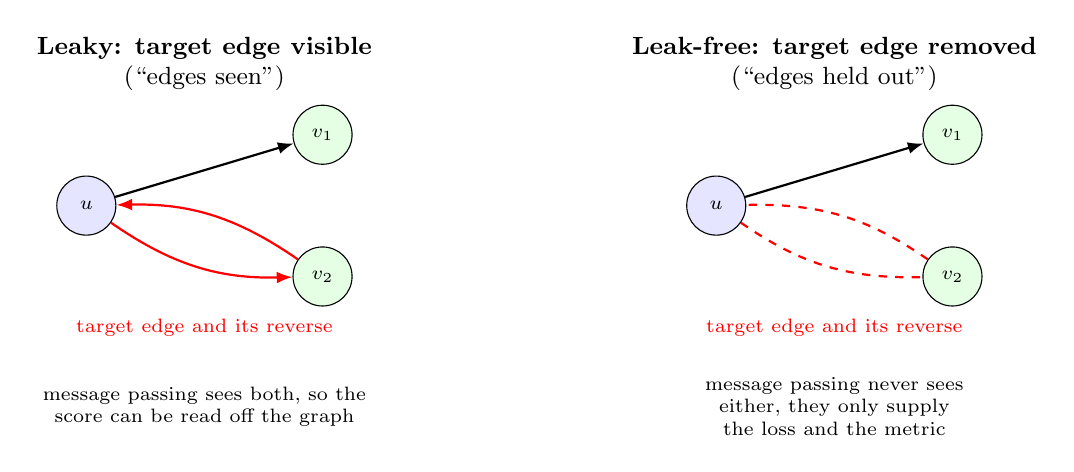
\begin{tikzpicture}[every node/.style={font=\scriptsize}]
\node[font=\small, align=center] at (1.5,3.3) {\textbf{Leaky: target edge visible}\\(``edges seen'')};
\node[draw, circle, fill=blue!10, minimum size=0.75cm] (m1) at (0,1.5) {$u$};
\node[draw, circle, fill=green!10, minimum size=0.75cm] (g1a) at (3.0,2.4) {$v_1$};
\node[draw, circle, fill=green!10, minimum size=0.75cm] (g1b) at (3.0,0.6) {$v_2$};
\draw[-{Latex[length=2mm]}, thick] (m1) -- (g1a);
\draw[-{Latex[length=2mm]}, thick, red, bend right=18] (m1) to (g1b);
\draw[-{Latex[length=2mm]}, thick, red, bend right=18] (g1b) to (m1);
\node[font=\scriptsize, text=red] at (1.5,-0.05) {target edge and its reverse};
\node[align=center, text width=4.2cm] at (1.5,-1.05) {message passing sees both, so the score can be read off the graph};

\node[font=\small, align=center] at (9.5,3.3) {\textbf{Leak-free: target edge removed}\\(``edges held out'')};
\node[draw, circle, fill=blue!10, minimum size=0.75cm] (m2) at (8,1.5) {$u$};
\node[draw, circle, fill=green!10, minimum size=0.75cm] (g2a) at (11.0,2.4) {$v_1$};
\node[draw, circle, fill=green!10, minimum size=0.75cm] (g2b) at (11.0,0.6) {$v_2$};
\draw[-{Latex[length=2mm]}, thick] (m2) -- (g2a);
\draw[dashed, thick, red, bend right=18] (m2) to (g2b);
\draw[dashed, thick, red, bend right=18] (g2b) to (m2);
\node[font=\scriptsize, text=red] at (9.5,-0.05) {target edge and its reverse};
\node[align=center, text width=4.2cm] at (9.5,-1.05) {message passing never sees either, they only supply the loss and the metric};
\end{tikzpicture}
\caption{Transductive edge leakage. A held-out edge and its reverse relation are either
visible to message passing (left) or removed before it (right). In our graph $u$ is a
miRNA and $v$ a gene.}
\label{fig:edge_split}
\end{figure}

\begin{figure}[h!]
\centering
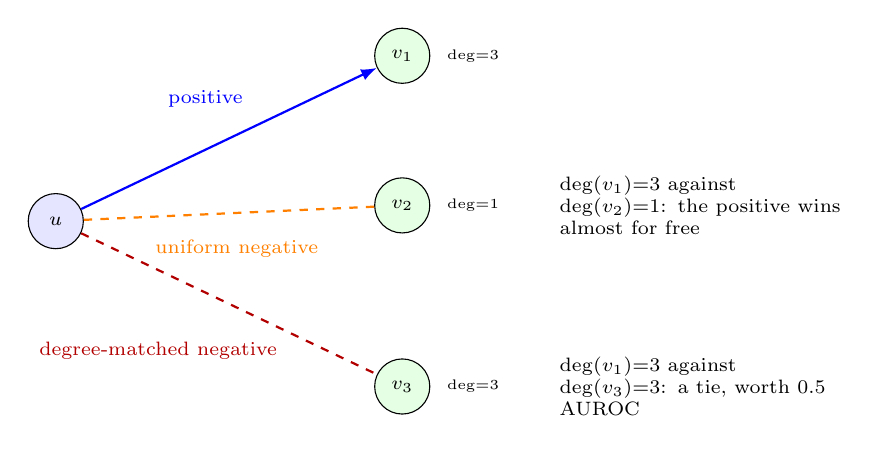
\begin{tikzpicture}[every node/.style={font=\scriptsize}]
\node[draw, circle, fill=blue!10, minimum size=0.7cm] (mm1) at (0,0) {$u$};
\node[draw, circle, fill=green!10, minimum size=0.7cm] (gg1) at (4.4,2.1) {$v_1$};
\node[font=\tiny] at (5.3,2.1) {deg=3};
\node[draw, circle, fill=green!10, minimum size=0.7cm] (gg2) at (4.4,0.2) {$v_2$};
\node[font=\tiny] at (5.3,0.2) {deg=1};
\node[draw, circle, fill=green!10, minimum size=0.7cm] (gg5) at (4.4,-2.1) {$v_3$};
\node[font=\tiny] at (5.3,-2.1) {deg=3};
\draw[-{Latex[length=2mm]}, thick, blue] (mm1) -- (gg1);
\node[font=\scriptsize, text=blue] at (1.9,1.55) {positive};
\draw[dashed, thick, orange] (mm1) -- (gg2);
\node[font=\scriptsize, text=orange] at (2.3,-0.35) {uniform negative};
\draw[dashed, thick, red!70!black] (mm1) -- (gg5);
\node[font=\scriptsize, text=red!70!black] at (1.3,-1.65) {degree-matched negative};
\node[align=left, text width=3.6cm] at (8.2,0.2) {$\deg(v_1){=}3$ against $\deg(v_2){=}1$: the positive wins almost for free};
\node[align=left, text width=3.6cm] at (8.2,-2.1) {$\deg(v_1){=}3$ against $\deg(v_3){=}3$: a tie, worth 0.5 AUROC};
\end{tikzpicture}
\caption{Popularity-biased negative sampling. For a scorer $\mathrm{score}(u,v)=\deg(v)$, a
uniform negative usually has lower degree than the positive's node and loses for free, while
a degree-matched negative ties.}
\label{fig:neg_sampling_mechanism}
\end{figure}

\begin{table}[h!]
\caption{Precedents for each element of the reporting standard. The first two pitfalls inflate a
reported number. The third is a reporting omission that leaves the inflation unseen.}
\label{tab:known_pitfalls}
\small
\begin{tabular}{>{\raggedright\arraybackslash}p{2.9cm}>{\raggedright\arraybackslash}p{4.0cm}>{\raggedright\arraybackslash}p{4.0cm}}
\hline
Pitfall & General ML / knowledge-graph precedent & Biomedical / network-biology precedent \\
\hline
Transductive edge leakage: message passing can see the held-out edge it is later
scored on. & Inverse-relation leak documented in the FB15k benchmark
\cite{toutanova2015observed}; actively re-examined in the broader link-prediction
literature \cite{zhu2023pitfalls,li2023evaluating}. & Independently identified in
miRNA--disease association prediction \cite{dong2020mirnaleakage}; train/test
redundancy shown to inflate knowledge-graph-embedding link prediction across several
biomedical graphs \cite{briere2026kgeleakage}. \\
Popularity-biased negative sampling: negatives drawn without regard to node degree
let a model win on popularity alone. & Known, quantified bias in link prediction
generally \cite{kotnis2017analysis,aiyappa2024implicit}; likely rooted in
recommender-systems evaluation practice \cite{krichene2020sampled}. & Documented
specifically in network biology \cite{yilmaz2025biasaware}, the domain this paper's
graph is drawn from. \\
Missing model-free baseline (a reporting omission): no model-free comparator, so a shortcut looks like learning. &
Topology-only methods can outperform GNN link predictors \cite{huang2023gelato}; OGB
lists heuristic baselines on its leaderboards \cite{ogb2026leaderboard}. & Common Neighbours
competitive with graph-embedding methods on small or sparse biomedical graphs
\cite{crichton2018realistic}. \\
\hline
\end{tabular}
\end{table}


\subsection{Evaluation practice in the literature}
Against that backdrop, we surveyed 21 papers in the miRNA-target and adjacent
biomolecule-interaction link-prediction literature (miRNA-disease, circRNA-disease,
lncRNA-disease, drug-target, and gene-disease), reading each paper's methods section in
full rather than inferring its protocol from the abstract
(Table~\ref{tab:literature_survey}). Three findings matter here. First, 14 of the 21
report no model-free baseline. The six that do report a classical untrained method as one
more competitor in a comparison table, never as a floor, and none remarks on how narrow
its margin over that comparator is. In the five papers whose numbers can be read from
the text, the headline clears the comparator by 1.7 to 7.4 AUROC points; NIMGSA's SPM
comparator (0.8960) comes within 3.9 points of NIMGSA itself (0.9354) and outscores IMCMDA
(0.8329), a trained baseline in the same table.
Second, 17 draw their negatives from unlabeled pairs, uniformly sampled or taken wholesale,
without discussing the alternative; only MGCNSS~\cite{tian2024mgcnss} and
HGDTI~\cite{yu2022hgdti} select them by a criterion of their own, and two papers never say.
Third, in 11 of the 19 papers where the question applies, it is unclear from the methods
section whether held-out edges are removed from the encoder's input. This is a reporting
gap, not confirmed leakage: after adjudication only MGCNSS clearly leaks and 7 clearly strip
test edges correctly, and our own project's original split was worse than the norm we
observed.

Getting the split right is not protective on its own. All seven papers that strip held-out
edges still draw their negatives from unlabeled pairs, none of them degree-matched, and four
of the seven report no model-free baseline. The two failure modes are independent, so fixing
the split is not evidence against the popularity-biased negative sampling this paper
identifies, which is why, as Results shows, correcting both is super-additive rather than
redundant.

\begin{table}[h!]
\caption{Literature survey (n=21): whether each paper removes held-out edges from the graph its model propagates over, how it chooses negative pairs, and whether it reports a model-free baseline. When it does, the cell names the untrained comparator and cites that method's original paper, not the surveyed one. The first six rows are the pilot sample; the other 15 are open-access (PMC) papers added later.}
\label{tab:literature_survey}
\footnotesize
\resizebox{\textwidth}{!}{%
\begin{tabular}{llcll}
\hline
Paper & Task & Held-out edges & Negative sampling & Model-free \\
 & & removed from graph? & & baseline \\
\hline
MGCNSS \cite{tian2024mgcnss} & miRNA-disease & no & distance-based selection (paper's own contribution) & no \\
NIMGSA \cite{jin2022nimgsa} & miRNA-disease & unclear & all unlabeled pairs (implicit: full-matrix loss) & SPM~\cite{lu2015spm} \\
HybridGNN \cite{ahmad2026hybridgnn} & miRNA-disease & yes & uniform random from unknown pairs & no \\
HGDTI \cite{yu2022hgdti} & drug-target & unclear & reliable score-filtered (non-uniform) & no \\
NGCN \cite{cao2024ngcn} & drug-target & yes & uniform random from unknown pairs, 1:10 & HNM~\cite{wang2014hnm} \\
kmerPMTF \cite{zhang2024kmerpmtf} & plant miRNA-target & unclear & all unlabeled pairs, count-matched & no \\
\hline
Orro \cite{orro2026mirnadisease} & miRNA-disease & yes (miRNA-level holdout) & uniform random from unannotated pairs & TCRWMDA~\cite{yu2020tcrwmda} \\
CoupleMDA \cite{li2025couplemda} & miRNA-disease & yes & uniform random, 1:1 & no \\
GONNMDA \cite{zeng2025gonnmda} & miRNA-disease & unclear & uniform random, 1:1 & no \\
DiGAMN \cite{liu2024digamn} & miRNA-disease & yes & uniform random, 1:1 / 1:5 / 1:10 & no \\
DGNMDA \cite{lu2024dgnmda} & miRNA-disease & unclear & uniform random from 0-labeled pairs, 1:1 & no \\
HLGNN-MDA \cite{yu2022hlgnnmda} & miRNA-disease & yes & uniform random, 1:1 & BNPMDA~\cite{chen2018bnpmda} \\
MEAHNE \cite{huang2022meahne} & miRNA-disease & unclear & uniform random, 1:1 & no \\
CKSNP-GNN \cite{li2022cksnpgnn} & miRNA-disease & unclear & uniform random, 1:1 & LLCMDA~\cite{qu2018llcmda} \\
HMCDA \cite{liang2023hmcda} & circRNA-disease & unclear & uniform random, 5:1 & no \\
HiGLDP \cite{wang2026higldp} & lncRNA-disease & unclear & not described (1:1 ratio only) & no \\
GPS-DTI \cite{xiong2025gpsdti} & drug-target & n/a$^{\dagger}$ & not described (balanced; 1--20$\times$ in the COVID-19 arm only) & no \\
SaeGraphDTI \cite{zhang2025saegraphdti} & drug-target & yes & all unlabeled pairs (unsampled) & no \\
DTI-MHAPR \cite{yang2025dtimhapr} & drug-target & unclear & uniform random, 1:1 & named (FSI), no result \\
iNGNN-DTI \cite{sun2024ingnndti} & drug-target & n/a$^{\dagger}$ & uniform random, 1:1 & no \\
ModulePred \cite{jia2024modulepred} & gene-disease & unclear & uniform random, 50:1 & RWR~\cite{tong2006rwr} \\
\hline
\end{tabular}
}

\medskip\par $^{\dagger}$iNGNN-DTI~\cite{sun2024ingnndti} and GPS-DTI~\cite{xiong2025gpsdti} encode drug and protein separately and never
propagate over a graph containing the predicted associations, so the held-out-edges
question does not apply to them (\S\ref{sec:methods}).
\end{table}


\section{Data and methods}
\label{sec:methods}

\subsection{Datasets}
\label{sec:data}
The claims in this paper rest on eight distinct graphs (Table~\ref{tab:datasets}).
The OGB counts are nodes and edges rather than matrix dimensions and positives, so those
columns are not comparable across groups. ``Retrained'' means our architecture is trained
under both protocol arms and ``heuristics'' that the model-free baselines are applied;
\S\ref{sec:comparison_design} describes how each graph is used.

\begin{table}[h!]
\caption{The eight distinct graphs used in this paper, with the matrix size and number of known associations (nodes and edges for OGB).}
\label{tab:datasets}
\footnotesize
\resizebox{\textwidth}{!}{%
\begin{tabular}{llccl}
\hline
Graph & Domain & Size & Positives & Used for \\
\hline
Our graph (miRDB v6.0~\cite{chen2020mirdb} + CELLxGENE scRNA-seq~\cite{czi2025cellxgene}) & miRNA--target & $2{,}460 \times 3{,}000$ & 44,186 & retrained, heuristics \\
\hline
Canonical HMDD~\cite{li2014hmdd} (MGCNSS~\cite{tian2024mgcnss}, NIMGSA~\cite{jin2022nimgsa}, HLGNN-MDA~\cite{yu2022hlgnnmda}) & miRNA--disease & $495 \times 383$ & 5,430 & retrained, heuristics \\
CKSNP-GNN~\cite{li2022cksnpgnn} & miRNA--disease & $901 \times 877$ & 16,427 & retrained, heuristics \\
DiGAMN~\cite{liu2024digamn} & miRNA--disease & $917 \times 792$ & 14,550 & retrained, heuristics \\
CoupleMDA~\cite{li2025couplemda} & miRNA--disease & $2{,}090 \times 1{,}754$ & 15,032 & retrained, heuristics \\
MEAHNE~\cite{huang2022meahne} & miRNA--disease & $1{,}296 \times 11{,}783$ & 17,972 & retrained, heuristics \\
\hline
ogbl-ddi \cite{hu2020ogb} & drug--drug & 4,267 nodes & 1,334,889 edges & heuristics \\
ogbl-ppa \cite{hu2020ogb} & protein--protein & 576,289 nodes & 30,326,273 edges & heuristics \\
\hline
\end{tabular}
}
\end{table}


\paragraph{External matrices and OGB} The five miRNA--disease matrices were recovered
from the papers surveyed in \S\ref{sec:related}; three of the seven papers whose data we
could obtain (MGCNSS, NIMGSA and HLGNN-MDA) share a byte-identical HMDD matrix. Each comes
from the paper's own repository, or a shared mirror for CKSNP-GNN, and was verified against
that paper's reported counts. Three further papers were excluded because no usable data was
recoverable (Discussion). ogbl-ddi and ogbl-ppa \cite{hu2020ogb} are public benchmarks with
open leaderboards, used only as an external check on the model-free baselines. In the
results table, only MGCNSS uses the paper's own exact test split (Tier 1); CoupleMDA's
positive edges are exact but its negatives are not (Tier 1/2); the other five HMDD rows use
an exact association matrix with a self-generated split at the paper's stated ratio (Tier 2).

\paragraph{Our graph} We build a heterogeneous graph from public multiple-sclerosis
single-cell RNA-seq data (blood, brain and cerebrospinal fluid) queried from the CZ
CELLxGENE Census (release 2025-11-08) \cite{czi2025cellxgene}, combined with miRDB v6.0
\cite{chen2020mirdb} miRNA--target interactions. It has three node types (miRNA, gene
and cell) joined by regulatory, expression and co-expression edges, each with a reverse
relation (Figure~\ref{fig:graph_schema}). After the fixes described below it has 2,460
miRNAs, 3,000 genes and 110,798 cells, with 44,186 miRNA$\to$gene, 16,682,321
cell$\to$gene and 828 gene--gene edges; Table~\ref{tab:datasets} counts miRNAs $\times$
genes, with the miRNA$\to$gene edges as positives. miRNA nodes carry a learnable
64-dimensional embedding (no prior biological signal), gene nodes the mean log-normalized
expression, and cell nodes a 50-dimensional PCA projection of their expression profile. The disease label attached to each cell is kept
only as provenance and never enters the graph, the model input, the objective or any
scoring head. We fixed two bugs in the graph-construction pipeline (co-expression gene
selection and the cell-to-gene expression threshold) and re-measured every headline number
on the corrected graph; all replicate the pre-fix figures within one standard deviation.

\begin{figure}[h!]
\centering
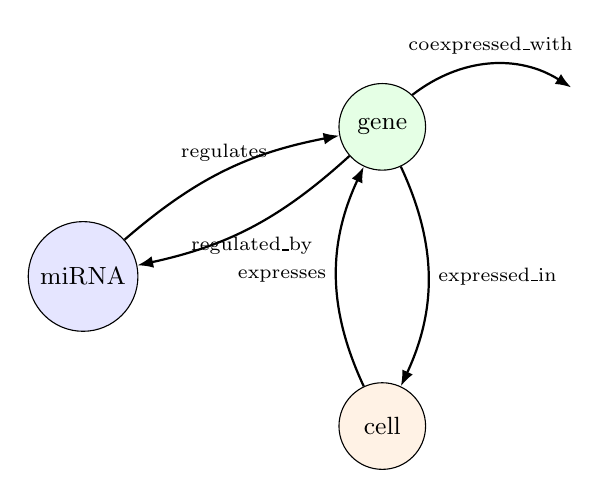
\begin{tikzpicture}[every node/.style={font=\small}]
\node[draw, circle, fill=blue!10, minimum size=1.1cm] (m) at (0,0) {miRNA};
\node[draw, circle, fill=green!10, minimum size=1.1cm] (g) at (3.8,1.9) {gene};
\node[draw, circle, fill=orange!10, minimum size=1.1cm] (c) at (3.8,-1.9) {cell};
\draw[-{Latex[length=2mm]}, thick, bend left=15] (m) to node[above, font=\scriptsize] {regulates} (g);
\draw[-{Latex[length=2mm]}, thick, bend left=15] (g) to node[below, font=\scriptsize] {regulated\_by} (m);
\draw[-{Latex[length=2mm]}, thick, bend left=25] (c) to node[left, font=\scriptsize] {expresses} (g);
\draw[-{Latex[length=2mm]}, thick, bend left=25] (g) to node[right, font=\scriptsize] {expressed\_in} (c);
\draw[-{Latex[length=2mm]}, thick, bend left=35] (g) to node[above, font=\scriptsize] {coexpressed\_with} +(2.4,0.5);
\end{tikzpicture}
\caption{Schema of our heterogeneous graph: three node types and three edge types, each with an automatically added reverse relation.}
\label{fig:graph_schema}
\end{figure}

\subsection{Evaluation protocol}
Link prediction scores node pairs $(u,v)$. Let $E$ be the set of target edges, the links
to predict: miRNA$\to$gene edges in our graph, miRNA--disease associations in the surveyed
matrices, and the benchmark's own edges in OGB. Any other edge types a graph has (in ours,
cell$\to$gene and gene--gene) are never held out. We evaluate every model under two
protocols. The \emph{conventional} protocol holds nothing out: every edge of $E$ stays in
the message-passing graph and is also a supervision and evaluation target (``edges
seen''), and negatives are drawn uniformly at random. The \emph{corrected} protocol holds test edges out of the message-passing graph and
draws degree-matched negatives. The data, labels, model and metric are the same in both. Crossing the two choices gives a $2\times2$ grid of edge
split by negative sampler (Figure~\ref{fig:protocol_grid} gives the four cells for our model), which lets us attribute the inflation to each failure
separately (\S\ref{sec:mechanism}). Table~\ref{tab:protocol_arms} gives the
difference between the two arms.

\begin{table}[h!]
\caption{What differs between the two protocols. $E$ is the set of target edges (the links to predict), $E_{\mathrm{tr}}$, $E_{\mathrm{va}}$ and $E_{\mathrm{te}}$ its training, validation and test parts, and $b(\cdot)$ the degree bin of a node (Eq.~\ref{eq:matched}). Data, labels, model and metric are identical.}
\label{tab:protocol_arms}
\small
\begin{tabular}{p{3.4cm}p{4.2cm}p{5.2cm}}
\hline
 & Conventional & Corrected \\
\hline
Message-passing graph & all of $E$ & $E_{\mathrm{tr}}$ only; $E_{\mathrm{va}}$, $E_{\mathrm{te}}$ and their reverse relations removed \\
Positives scored & all of $E$, which are also the training targets & $E_{\mathrm{te}}$, never seen by the encoder \\
Negative $(u,v')$ for a positive $(u,v)$ & $v'$ drawn uniformly at random & $v'$ with $b(v')=b(v)$ \\
\hline
\end{tabular}
\end{table}


We use \emph{transductive edge leakage} for the specific condition audited here: a
held-out edge left in the message-passing graph when its score is computed, so the
encoder can, in effect, observe the edge it is later asked to predict, narrower than
the general transductive/inductive distinction in graph learning, which is not itself a
source of leakage. In the corrected protocol, 10\% of the edges of $E$ are held
out for validation and 10\% for testing at random, and each held-out edge, with its
automatically-added reverse relation, is removed from the message-passing graph in both
directions. An automated battery of checks verifies this before any downstream number is
trusted (Figure~\ref{fig:edge_split}). The same logic applies within the training set: 30\%
of the training edges are withheld from the encoder's input and used only as supervision
targets, so the model cannot read a training edge off the graph while being asked to
predict it.

A uniform negative pairs the source node $u$ of a positive with a target node drawn
uniformly at random. A degree-matched negative pairs it instead with a non-target node of
similar popularity: target nodes are placed in eight log-spaced bins of in-degree,
computed from training edges only, and each positive $(u,v)$ receives a negative $(u,v')$
with $v'$ in the same bin as $v$:
\begin{equation}
v' \sim \mathcal{U}\bigl\{\, j : b(j) = b(v),\ (u,j)\notin E \,\bigr\},
\qquad b(j)=\mathrm{bin}_8\bigl(\log(1+d_{\mathrm{tr}}(j))\bigr),
\label{eq:matched}
\end{equation}
where $d_{\mathrm{tr}}(j)$ is the in-degree of node $j$ among training edges.
When no valid candidate is found in 16 draws the sampler falls back to any non-target of
$u$, and the fraction of fallbacks is logged. Within any single reported number the same
sampler is used at training and at evaluation; mixing the two produces the ``mismatch
trap'', an apparent difficulty measurement that is in fact an artifact of the distribution
mismatch (Figure~\ref{fig:neg_sampling_mechanism}). In the headline grid
(Figure~\ref{fig:protocol_grid}), the edges-seen row reports the uniform-negative-trained model
under both evaluation regimes, and the edges-held-out row each model scored with the negative
type it was trained on. The third requirement of the standard we
propose concerns reporting rather than the protocol itself: a model-free baseline, whose
margin over the trained model is stated alongside the headline number
(\S\ref{sec:baselines}).

We report AUROC and AUPRC for link prediction, and accuracy and macro-F1 for cell
typing, averaged over four random seeds where feasible. The model grid is a
single run per model, on one GPU, by a driver separate from the multi-GPU
headline runs; Results gives the effect-size argument for the single run and the
comparability limit the driver difference imposes.

%% RESOLVED (2026-10-12): the minimum-reporting checklist (tab:correct_protocol) lives in the Discussion,
%% in the subsection on the standard and protocheck (sec:standard), with the validation paragraph.

\subsection{Experimental design}
\label{sec:comparison_design}
The protocol defined above is applied in seven experiments (Table~\ref{tab:experiments}),
ordered as Results reports them. E1--E4 compare graphs and papers, so that whether the
inflation is a property of the protocol rather than of any single graph or model can be
measured rather than assumed; our own graph (\S\ref{sec:data}) is one case among them, not
the case they are built around. Together they cover ten cases (our graph, seven surveyed
papers and two OGB benchmarks) on eight distinct graphs, because three of the papers
share one matrix. E5 asks what separates the graphs, and E6 and E7 use the one graph whose
construction and training we control: E6 asks why the inflation arises, and E7 asks whether the
audit also deflates a different task on that graph, cell typing, which is not link prediction.

\begin{table}[h!]
\caption{The seven experiments (E1--E7 are experiments 1--7), in the order Results reports them. ``Six graphs'' are ours, the canonical HMDD matrix (shared by MGCNSS, NIMGSA and HLGNN-MDA), CKSNP-GNN, DiGAMN, CoupleMDA and MEAHNE; the five external matrices are the last five. The grid is the $2\times2$ of edge split by negative sampler.}
\label{tab:experiments}
\footnotesize
{\setlength{\tabcolsep}{3pt}
\begin{tabular}{p{0.5cm}p{2.8cm}p{3.3cm}p{3.2cm}p{0.9cm}}
\hline
 & Question & Data & What is run & Results \\
\hline
E1 & Does the collapse occur on other graphs? & The six graphs & Our architecture retrained from scratch under both protocol arms, mean over four seeds & \S\ref{sec:collapse_general} \\
E2 & How much does each failure contribute without a trained model? & The six graphs & The four model-free heuristics across the full grid & \S\ref{sec:collapse_general} \\
E3 & How far above a model-free floor are published numbers? & The five external matrices, i.e.\ the seven surveyed papers (MGCNSS, NIMGSA, HLGNN-MDA, CKSNP-GNN, DiGAMN, CoupleMDA, MEAHNE) & The heuristics, unmodified, under each paper's negative ratio, read against its published number & \S\ref{sec:generalization} \\
E4 & Does the floor behave the same outside this literature? & ogbl-ddi, ogbl-ppa & The same heuristics after a runtime leak-free check, read against the public leaderboards & \S\ref{sec:generalization} \\
E5 & What separates the graphs? & The five external matrices (thinning); the canonical HMDD matrix (padding) & Positives thinned from 100\% to 10\% (five seeds per point); empty candidate columns added; model-free floor measured & \S\ref{sec:dead_columns} \\
E6 & Does the inflation follow the protocol or the model? & Our graph (CZ CELLxGENE Census scRNA-seq with miRDB v6.0) & The transformer over the full grid (four seeds); four trained models and an untrained control over the grid (one run each) & \S\ref{sec:mechanism} \\
E7 & Does the audit deflate a task that is not leaky? & Our graph, cell-type labels of its cells & The trained model against two graph-free controls & \S\ref{sec:celltype} \\
\hline
\end{tabular}}
\end{table}


\subsection{Baselines and models}
\label{sec:baselines}
\paragraph{Model-free baselines} A model-free baseline is a comparator that does not use
the machinery of the model under test. Its score is the floor a trained model must clear,
and the margin is the model's score minus that floor. In link prediction it is a
parameter-free topological heuristic: it ranks candidate pairs from the training-visible
structure of the graph alone, so it measures how much of a reported AUROC the topology
already provides. We use four (Table~\ref{tab:heuristics}), computed on the training edges
only, and call them the model-free heuristics; the model-free floor on a graph is the AUROC
of the best of them. Gene in-degree doubles as a sanity check: against degree-matched
negatives it should sit near 0.5 by construction. On the external matrices the floor is an
AUROC, and on OGB it is Hits@$K$, the metric of the public leaderboards. For cell typing
the equivalent comparator is a graph-free classifier on the same input features: nearest
centroid, which has no fitted parameters beyond the class means, and logistic regression, a
fitted linear model, both trained directly on the raw PCA features without message passing.

\begin{table}[h!]
\caption{The four model-free heuristics. $A$ is the adjacency of the training edges of $E$, $N(u)$ the neighbours of $u$, and $d(\cdot)$ the degree.}
\label{tab:heuristics}
\small
\begin{tabular}{p{3.2cm}p{5.3cm}p{3.6cm}}
\hline
Heuristic & Score of a pair $(u,v)$ & Reads as \\
\hline
Gene in-degree & $d(v)$ & the popularity of $v$ \\
Preferential attachment & $d(u)\,d(v)$ & popularity of both ends \\
Common neighbours & $\sum_{u'\neq u} |N(u)\cap N(u')|\,A_{u'v}$ & how much $u$ shares targets with the nodes that reach $v$ \\
Adamic--Adar & $\sum_{u'\neq u}\sum_{w\in N(u)\cap N(u')} A_{u'v}/\log d(w)$ & the same, down-weighting shared targets that everything reaches \\
\hline
\end{tabular}
\end{table}


\paragraph{Models} The link-prediction experiments compare these baselines with four
trained models (a heterogeneous graph transformer, a homogeneous GCN, a
co-expression-ablation variant of the transformer, and a graph-free MLP) plus an
untrained random-weight control.

\section{Results}
\label{sec:results}
Table~\ref{tab:results_summary} gives the main result of each of the seven experiments; the
subsections below follow the same order.

\begin{table}[!t]
\caption{The main result of each experiment (E1--E7, Table~\ref{tab:experiments}).}
\label{tab:results_summary}
\footnotesize
{\setlength{\tabcolsep}{3pt}
\newcolumntype{R}[1]{>{\raggedright\arraybackslash}p{#1}}
\begin{tabular}{R{0.5cm}R{8.6cm}R{1.4cm}}
\hline
 & Main result & Section \\
\hline
E1 & AUROC falls from 0.879--0.992 to 0.618--0.641 on all six graphs, a loss of 0.26--0.37 on each & \S\ref{sec:collapse_general} \\
E2 & The model-free heuristics inflate by 0.32--0.43; negative sampling carries about 0.30 and the split 0.01--0.02 on the five surveyed graphs & \S\ref{sec:collapse_general} \\
E3 & Trained models beat the model-free floor by 4.7 points per paper, from $-9.2$ to $+3.3$ & \S\ref{sec:generalization} \\
E4 & The heuristics reproduce the leaderboards: 30th of 32 on ogbl-ddi, 14th of 27 on ogbl-ppa~\cite{ogb2026leaderboard} & \S\ref{sec:generalization} \\
E5 & Empty candidate columns alone raise the floor from 0.859 to 0.982 & \S\ref{sec:dead_columns} \\
E6 & On our graph the transformer falls from 0.9867 to 0.6276, and four trained models inflate by 0.24--0.31 while the untrained control does not move & \S\ref{sec:mechanism} \\
E7 & Cell typing reaches 0.9916 against 0.4654 and 0.6692 for the graph-free controls, a 32-point gap, so the audit leaves it intact & \S\ref{sec:celltype} \\
\hline
\end{tabular}}
\end{table}


\subsection{Inflation across six graphs (E1, E2)}
\label{sec:collapse_general}
We retrain this paper's architecture from scratch under both protocols on six graphs
(Figure~\ref{fig:cross_graph_collapse}, Table~\ref{tab:discrimination}). AUROC falls from
0.879--0.992 under the conventional protocol to 0.618--0.641 once test edges are held out
and negatives are degree-matched, an inflation of 0.256 to 0.365 on every graph. Six graphs
that share no data, no node types and no size land in the same 0.023-wide band. Our own
graph's $+0.359$ is inside that range, near its upper end: it is a member of the
distribution, not an outlier. The trained arm is our architecture on their graphs, not each
paper's own model, so the table is evidence about the protocol, not about their reported
numbers (Discussion).

\begin{figure}[h!]
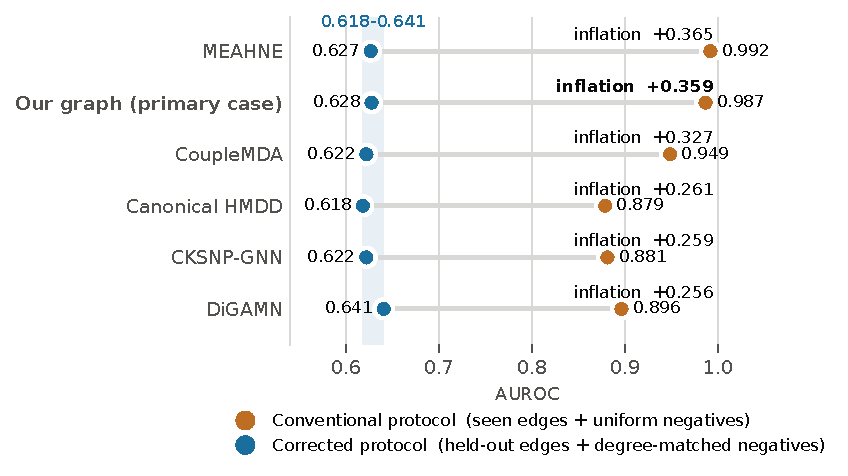
\includegraphics[width=\textwidth]{../../results/figures/manuscript/fig4_cross_graph_collapse.pdf}
\caption{The same inflation on six graphs: this paper's architecture under the conventional and corrected protocols (mean over 4 seeds). Rows are sorted by inflation, our graph is in bold, and the band marks 0.618--0.641.}
\label{fig:cross_graph_collapse}
\end{figure}

\begin{table}[h!]
\caption{The inflation on every graph with a trained protocol grid (our architecture, mean of 4 seeds), and its margin over the best model-free heuristic. Conventional = edges seen, uniform negatives; corrected = edges held out, degree-matched negatives.}
\label{tab:discrimination}
\footnotesize
\resizebox{\textwidth}{!}{%
\begin{tabular}{lcccccc}
\hline
 & \multicolumn{3}{c}{Conventional protocol} & \multicolumn{3}{c}{Corrected protocol} \\
\cline{2-4}\cline{5-7}
Graph & Our architecture & Model-free & Margin & Our architecture & Model-free & Margin \\
\hline
Own graph (primary case) & 0.9867 & 0.9336 & $+0.0531$ & 0.6276 & 0.5912 & $+0.0364$ \\
\hline
Canonical HMDD & 0.8789 & 0.8842 & $-0.0053$ & 0.6182 & 0.5683 & $+0.0499$ \\
CKSNP-GNN & 0.8812 & 0.8924 & $-0.0112$ & 0.6219 & 0.5591 & $+0.0628$ \\
DiGAMN & 0.8963 & 0.8833 & $+0.0130$ & 0.6406 & 0.5580 & $+0.0826$ \\
MEAHNE & 0.9919 & 0.9908 & $+0.0012$ & 0.6266 & 0.5648 & $+0.0618$ \\
CoupleMDA & 0.9487 & 0.9497 & $-0.0010$ & 0.6220 & 0.5789 & $+0.0431$ \\
\hline
\end{tabular}
}
\end{table}


Running the same $2\times2$ grid (Figure~\ref{fig:protocol_grid}) with the four model-free
heuristics (Table~\ref{tab:heuristics}) instead of a trained model
(Table~\ref{tab:protocol_grid}, in \S\ref{sec:dead_columns}) shows the inflation is not something only a trained model
produces. Within a row only the adjacency the heuristics may see changes, so the inflation
is attributable to the protocol alone: $+0.316$ to $+0.426$ across the six graphs, with our
graph's $+0.342$ inside the range. How it divides between the two failures differs. On the
five surveyed graphs the negative-sampling axis carries almost the whole effect
($\approx 0.30$) and the edge split only $0.01$--$0.02$, because these association matrices
are small and their heuristics lean on node degree, which a handful of masked edges barely
moves. On our own graph the two axes are comparable and compound super-additively. The
canonical HMDD matrix appears twice because MGCNSS is scored on its own bundled split, and
MGCNSS has no negative-sampling axis because it carries the paper's own negatives.

One asymmetry in Table~\ref{tab:discrimination} is measured but not explained. On the five
surveyed graphs the conventional protocol leaves the trained model within 1.3 points of the
best heuristic, behind it on three, and the corrected protocol opens that margin to between
4.3 and 8.3 points, so only the corrected one can tell a trained model from a degree count.
On our graph the margin narrows from $+0.053$ to $+0.036$. The obvious explanation, that our
node features and miRNA embeddings let the model memorise training edges under the
conventional protocol, does not hold: per-epoch training and validation loss show the same
divergence on all six graphs, including the five with nothing to memorise. We report it as an
open observation, like the candidate-space correlation in \S\ref{sec:dead_columns}. It does
not affect the figures, since every checkpoint is selected at peak validation AUROC, before
that divergence begins.

\subsection{Published results against a model-free floor (E3, E4)}
\label{sec:generalization}
Table~\ref{tab:validation_cases} gives the ten cases, and three results stand out. First, on
the seven surveyed papers' own matrices the trained models beat the model-free floor by 4.7
AUROC points on average per paper (3.9 per distinct graph), but the gap runs from $-9.2$
points (DiGAMN) to $+3.3$: on MEAHNE's graph the heuristic beats the paper's own model
(0.9848 vs.\ 0.9520), and with degree-matched negatives every heuristic falls to
0.55--0.58. Second, the floor replicates. The untrained comparators that NIMGSA, HLGNN-MDA
and CKSNP-GNN report (0.8960, 0.8565 and 0.9190) sit beside the 0.8842 and 0.8924 that our
best heuristic reaches on their matrices under the conventional protocol, and CKSNP-GNN's
is a number transferred from other papers, not measured on its own data. Third, on OGB the
heuristics reproduce the leaderboards exactly and the floor is not uniform: on ogbl-ddi the
best heuristic ranks 30th of 32, while on ogbl-ppa a zero-parameter formula ranks 14th of 27,
essentially tied with the entry just above it, BUDDY \cite{chamberlain2023buddy} (0.4933 vs.\
0.4934 Hits@100).

\begin{table}[h!]
\caption{Model-free baselines on all ten cases: our graph, two OGB benchmarks \cite{hu2020ogb} and seven surveyed papers' datasets. ``Best reported'' is the paper's own model under its own protocol; ``Model-free'' is the best of the four heuristics with test edges held out and uniform negatives (the own-graph row uses the corrected protocol and is excluded from the means). AUROC and Hits@$K$ rows are not comparable.}
\label{tab:validation_cases}
\footnotesize
\resizebox{\textwidth}{!}{%
\begin{tabular}{llllccc}
\hline
Case & Domain & Metric & Best reported (their model) & Model-free (best) & Gap & Rank of model-free \\
\hline
Own graph (primary case) & miRNA--target & AUROC & 0.6276 & 0.5912 (Adamic--Adar) & $-0.0365$ & -- \\
\hline
ogbl-ddi \cite{hu2020ogb} & drug--drug & Hits@20 & 0.9972 (HyperFusion) & 0.1861 (Adamic--Adar) & $-0.811$ & 30 / 32 \\
ogbl-ppa \cite{hu2020ogb} & protein--protein & Hits@100 & 0.4934 (BUDDY \cite{chamberlain2023buddy}) & 0.4933 (Resource Alloc.) & $-0.0001$ & 14 / 27 \\
\hline
\multicolumn{7}{l}{\emph{Shared canonical HMDD matrix (495 $\times$ 383, 5,430 associations) -- one graph, three papers}} \\
MGCNSS \cite{tian2024mgcnss} & miRNA-disease & AUROC & 0.9874 & 0.9136 & $-0.074$ & Tier 1 \\
NIMGSA \cite{jin2022nimgsa} & miRNA-disease & AUROC & 0.9354 & 0.8680 & $-0.067$ & Tier 2 \\
HLGNN-MDA \cite{yu2022hlgnnmda} & miRNA-disease & AUROC & 0.93086 & 0.8680 & $-0.063$ & Tier 2 \\
\multicolumn{7}{l}{\emph{Distinct graphs, one paper each}} \\
DiGAMN \cite{liu2024digamn} & miRNA-disease & AUROC & 0.9635 & 0.8714 & $-0.092$ & Tier 2 \\
CoupleMDA \cite{li2025couplemda} & miRNA-disease & AUROC & 0.9536 & 0.9406 & $-0.013$ & Tier 1/2 \\
MEAHNE \cite{huang2022meahne} & miRNA-disease & AUROC & 0.9520 & \textbf{0.9848} & $\mathbf{+0.033}$ & Tier 2 \\
CKSNP-GNN \cite{li2022cksnpgnn} & miRNA-disease & AUROC & 0.9371 & 0.8822 & $-0.055$ & Tier 2 \\
\hline
Mean, 7 surveyed papers & & AUROC & 0.951 & 0.905 & $-0.047$ & \\
Mean, 5 distinct graphs & & AUROC & 0.951 & 0.912 & $-0.039$ & \\
\hline
\end{tabular}
}
\end{table}


\subsection{Why the floor is high on some graphs: empty columns (E5)}
\label{sec:dead_columns}
In a miRNA--disease matrix the columns are the diseases a miRNA can be paired with, and a
column is \emph{empty} when no association is known for it, so it can never be a positive.
Under uniform negatives such columns supply negatives that any scorer aware of degree
rejects for free. MEAHNE has 11{,}783 disease columns, 92.4\% of them empty, and CoupleMDA
55.7\%, while the other three external graphs have none (Table~\ref{tab:protocol_grid}).

\begin{table}[h!]
\caption{The model-free protocol grid: best of the four heuristics in each cell, on our graph and on each distinct graph behind the surveyed papers. Inflation is the seen, uniform cell minus the held-out, degree-matched one. Empty and Gini are defined in \S\ref{sec:data}.}
\label{tab:protocol_grid}
\footnotesize
\resizebox{\textwidth}{!}{%
\begin{tabular}{llccccccc}
\hline
 & & & & \multicolumn{2}{c}{Uniform negatives} & \multicolumn{2}{c}{Degree-matched} & \\
\cline{5-6}\cline{7-8}
Graph & Paper(s) & Empty & Gini & seen & held out & seen & held out & Inflation \\
\hline
Own graph (primary case) & -- & 47.5\% & 0.742 & 0.9336 & 0.8712 & 0.7237 & 0.5912 & $+0.342$ \\
Canonical HMDD~\cite{li2014hmdd}, paper's split & MGCNSS~\cite{tian2024mgcnss} & 0.0\% & 0.712 & 0.9613 & 0.9136 & -- & -- & $+0.048$ \\
Canonical HMDD, generated split & NIMGSA~\cite{jin2022nimgsa}, HLGNN-MDA~\cite{yu2022hlgnnmda} & 0.0\% & 0.712 & 0.8842 & 0.8680 & 0.5986 & 0.5683 & $+0.316$ \\
DiGAMN & DiGAMN~\cite{liu2024digamn} & 0.0\% & 0.723 & 0.8833 & 0.8714 & 0.5756 & 0.5580 & $+0.325$ \\
CKSNP-GNN & CKSNP-GNN~\cite{li2022cksnpgnn} & 0.0\% & 0.713 & 0.8924 & 0.8822 & 0.5746 & 0.5591 & $+0.333$ \\
CoupleMDA & CoupleMDA~\cite{li2025couplemda} & 55.7\% & 0.874 & 0.9497 & 0.9406 & 0.5944 & 0.5789 & $+0.371$ \\
MEAHNE & MEAHNE~\cite{huang2022meahne} & 92.4\% & 0.979 & 0.9908 & 0.9848 & 0.5813 & 0.5648 & $+0.426$ \\
\hline
\end{tabular}
}
\end{table}


Sparsity is not the explanation: thinning the positives of each graph lowers the
model-free floor on all five external graphs (Spearman $\rho = +0.60$ to $+1.00$ against
density) instead of raising it. Across the six graphs no descriptive statistic separates
them significantly (empty-column fraction $\rho = +0.70$, $p = 0.12$; column-degree Gini
$\rho = +0.77$, $p = 0.07$), and our own graph is a counterexample, with 47.5\% empty columns
and a floor indistinguishable from the graphs with none. The direct evidence is a
manipulation. Adding empty columns to the canonical HMDD matrix, which has none, and nothing
else, raises its model-free floor from $0.859 \pm 0.014$ to $0.982 \pm 0.006$. At 92.9\%
empty columns, MEAHNE's own level, it reaches $0.979$, reproducing MEAHNE's outlying $0.9848$
from a graph that shares none of its data.

\subsection{Sources of the inflation on our graph (E6)}
\label{sec:mechanism}
The two corrections are not redundant. From the conventional 0.9867, matched negatives alone
lower AUROC by 0.062 and held-out edges alone by 0.177, a sum of 0.239, while together they
lower it by 0.359 (Figure~\ref{fig:protocol_grid}): the pair
is super-additive. How the total divides depends on which is applied first (the negatives
lower it by 0.062 with edges seen but 0.182 with edges held out), so we report the total
rather than a decomposition.

\begin{figure}[h!]
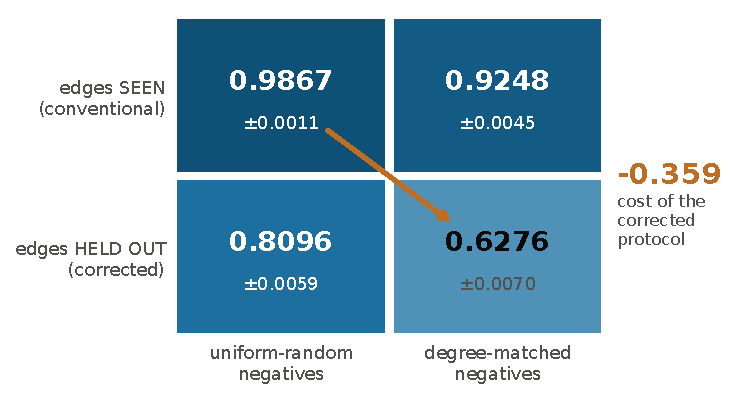
\includegraphics[width=\textwidth]{../../results/figures/manuscript/fig1_protocol_grid.pdf}
\caption{Headline protocol grid: AUROC (mean $\pm$ std, 4 seeds) by edge split and negative sampler.}
\label{fig:protocol_grid}
\end{figure}

A model trained with uniform negatives and scored against degree-matched ones falls to AUROC
$0.5352 \pm 0.0202$, indistinguishable from the in-degree floor (Table~\ref{tab:model_free_baselines}), so
uniform-negative training teaches popularity rather than miRNA-specific target information. The same
fall occurs in every trained architecture in the grid (Figure~\ref{fig:negative_sampler_collapse}).

\begin{figure}[h!]
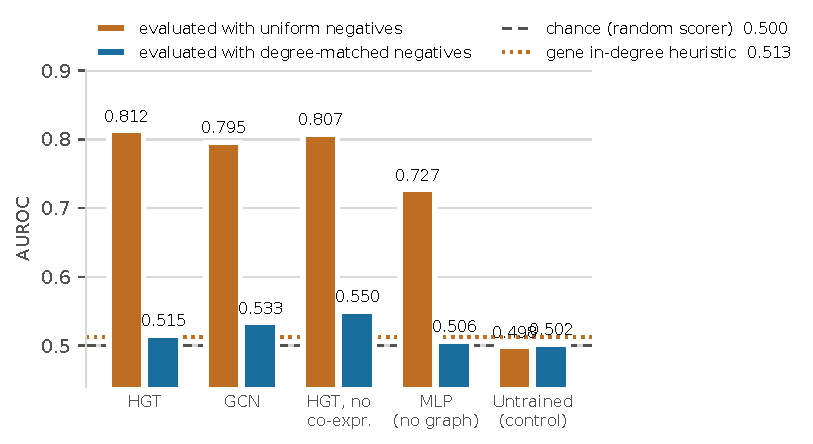
\includegraphics[width=\textwidth]{../../results/figures/manuscript/fig3_negative_sampler_collapse.pdf}
\caption{Every architecture trained with uniform negatives, scored under both regimes. Chance is a random scorer; the gene in-degree heuristic is in Table~\ref{tab:heuristics}.}
\label{fig:negative_sampler_collapse}
\end{figure}

\begin{table}[h!]
\caption{Model-free heuristics versus the trained model on held-out test edges (\texttt{graphs\_v3fixed}; trained rows are mean $\pm$ std over 4 seeds, the heuristics are deterministic). $^{\dagger}$The uniform-trained model scored against degree-matched negatives: a distribution mismatch, not a difficulty measurement (\S\ref{sec:methods}).}
\label{tab:model_free_baselines}
\small
\begin{tabular}{lcc}
\hline
Heuristic & Uniform negatives & Degree-matched negatives \\
\hline
Gene in-degree (ignores the miRNA) & 0.8712 & 0.5126 \\
Preferential attachment & 0.8381 & 0.5074 \\
Common neighbours & 0.8597 & 0.5840 \\
Adamic--Adar (best heuristic) & 0.8630 & 0.5912 \\
\hline
HGT, trained with uniform negatives & 0.8096 $\pm$ 0.0059 & 0.5352 $\pm$ 0.0202 $\dagger$ \\
HGT, trained with degree-matched negatives & 0.5642 $\pm$ 0.0052 $\dagger$ & 0.6276 $\pm$ 0.0070 \\
\hline
\end{tabular}
\end{table}


Nor is the inflation specific to one model. Four trained models (the transformer, a
homogeneous GCN, a co-expression ablation and a graph-free MLP) inflate by 0.24--0.31 AUROC
between the two protocols, the MLP included, while an untrained random-weight control does
not move ($-0.004$; Figure~\ref{fig:architecture_inflation}). Each is a single run on one GPU,
so the levels are comparable with one another but not with Figure~\ref{fig:protocol_grid}
(\ref{app:grid}).

\begin{figure}[h!]
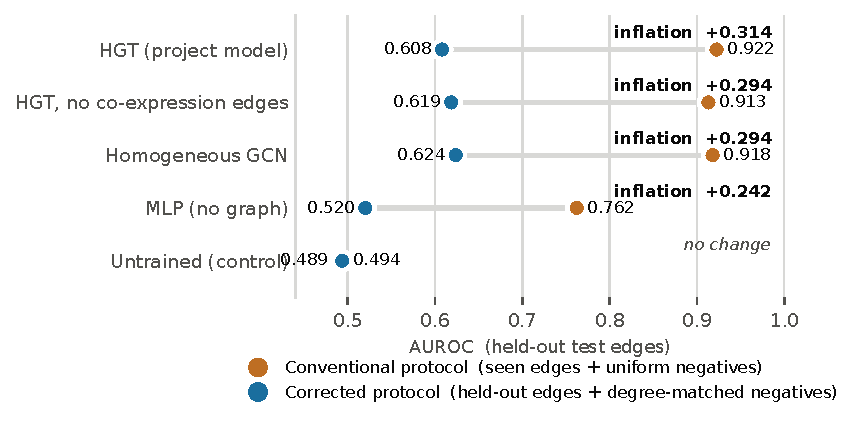
\includegraphics[width=\textwidth]{../../results/figures/manuscript/fig2_architecture_inflation.pdf}
\caption{Inflation across four trained models and an untrained control (single seed, one GPU; \ref{app:grid}).}
\label{fig:architecture_inflation}
\end{figure}

\subsection{Cell-type classification control (E7)}
\label{sec:celltype}
The audit does not deflate every number it touches. This control moves from link prediction to a
different task on the same graph: classifying the cell type of each cell (node classification). The
label of a cell is the highest marker-gene score computed from its expression, and the only cell
feature the model sees is a PCA of that same expression, so the 0.9916 test accuracy could
be the model recomputing its own label. Two graph-free controls on the PCA features alone, with no
graph and no message passing, test this: nearest-centroid reaches 0.4654 and logistic regression
0.6692 (Table~\ref{tab:celltype_control}). The trained model's gap to the better control, 32 points,
is an order of magnitude larger than the 3.6 points the corrected link-prediction protocol leaves
between the trained model and its topological floor. Here the graph and message passing do
substantial work, and the same methodology leaves the number intact: the audit is
discriminating rather than indiscriminate.

\begin{table}[h!]
\caption{Cell-type classification: graph-free controls (nearest-centroid, logistic regression, both on \texttt{X\_pca} alone, no message passing) vs.\ the trained HGT, same split/config/seed, test set. Source: configs/config\_v2\_edgesplit.yaml, n=11079 held-out cells.}
\label{tab:celltype_control}
\small
\begin{tabular}{lcc}
\hline
Classifier & Accuracy & Macro-F1 \\
\hline
Nearest-centroid (graph-free) & 0.4654 & 0.4612 \\
Logistic regression (graph-free) & 0.6692 & 0.5737 \\
HGT (reference, degree-matched) & 0.9916 & -- \\
\hline
\end{tabular}
\end{table}


\section{Discussion}
\label{sec:discussion}

Collapsing to chance the moment gene in-degree is closed off (Table~\ref{tab:model_free_baselines}) is the
signature of shortcut learning \cite{geirhos2020shortcut}, not of a harder evaluation. What we have not found
named in the literature is the interaction between the two failures: prior work studies transductive edge leakage
or popularity-biased negative sampling in isolation (Section~\ref{sec:related}, Table~\ref{tab:known_pitfalls}),
but on our graph they are super-additive (Figure~\ref{fig:protocol_grid}), so auditing for one and not the other
can still miss an inflated headline. We call this \emph{compounded evaluation inflation}. Empty candidate
columns act through the second failure: under uniform negatives they supply negatives that any degree-aware
scorer rejects for free, raising the model-free floor from 0.859 to 0.982 with no learning
(Section~\ref{sec:dead_columns}). The model-free baseline is not a third source of inflation; it is what makes
the other two visible.

None of this is specific to our graph or to one model. Five external association matrices that share no data
with ours each lose 0.26--0.37 AUROC between the protocols and land in the same 0.618--0.641 band
(Table~\ref{tab:discrimination}); four trained models inflate by 0.24--0.31 while an untrained control does not
move, and cell typing on the same graph survives the same audit by 32 points (Section~\ref{sec:celltype}). The
weakness against a floor also appears in published work. Across the seven surveyed papers the trained models
beat the floor by 4.7 points on average, from 9.2 points above it (DiGAMN) to 3.3 below it (MEAHNE), and on
ogbl-ppa a zero-parameter formula ranks 14th of 27, tied with BUDDY. OGB already reports such heuristics, and the
gap persists, so reporting a baseline does not by itself raise the bar. A headline within a few points of the
floor is hard to read as evidence of learning.

\subsection{A minimum reporting standard and \texttt{protocheck}}
\label{sec:standard}
Given how directly the inflation problem responds to a small set of checks, we propose these as a minimum reporting standard for evaluation methodology in this subfield. First, a leak-free edge split, with an automated check that held-out edges are unreachable to the encoder during message passing. Second, matched negative sampling: negative-sampling distributions that are matched between training and evaluation rather than assumed compatible. Third, at least one model-free baseline reported alongside any trained model, \emph{and the margin over it stated}. Six of the surveyed papers report such a comparator and none reads its own margin. We release \texttt{protocheck}, a tool that verifies whether an evaluation meets the standard on the user's own splits. Table~\ref{tab:correct_protocol} gives the three requirements and the check of \texttt{protocheck} that verifies each.

\begin{table}[h!]
\caption{Minimum reporting checklist for link-prediction models on biomedical interaction graphs. The first two requirements prevent two independent protocol failures; the third is a reporting requirement. Each has a check in \texttt{protocheck}.}
\label{tab:correct_protocol}
\small
\begin{tabular}{p{3.1cm}p{4.7cm}p{5.4cm}}
\hline
Requirement & Problem it prevents & How this study implements it \\
\hline
Leak-free edge split & Transductive edge leakage: the encoder can recover a held-out
edge from its own neighborhood (Figure~\ref{fig:edge_split}). & Held-out edges and
their reverse relation are stripped from the message-passing graph; an automated
test verifies none is reachable. \\
Matched negative sampling & Popularity-biased negative sampling and
the ``mismatch trap'': evaluating against a different negative distribution than
trained on produces an artifact, not a difficulty measurement (Figure~\ref{fig:neg_sampling_mechanism}). & The same
sampler (uniform-random or degree-matched) is enforced at training and evaluation
for every reported number. \\
Model-free baseline, with its margin stated & Reporting omission: without a model-free comparator, a model that learned a
trivial shortcut (e.g.\ popularity) is indistinguishable from one that learned the
task (Table~\ref{tab:model_free_baselines}). & A topological heuristic (link
prediction) or non-graph classifier (node classification) is reported alongside
every trained model, under the same protocol. \\
\hline
\end{tabular}
\end{table}


\texttt{protocheck} takes the train and held-out pairs of a link-prediction experiment and, optionally, the edges the encoder sees, the training and evaluation negatives and the model's AUROC. It reports each check as ok, warn or fail; a check whose input was not supplied is reported as unchecked, never as passed. It needs only numpy, scipy and scikit-learn, and runs from the command line, from Python, or in a Colab notebook on the user's own files (Data availability). It also runs a fourth, diagnostic check for candidate columns that carry no positive anywhere (Section~\ref{sec:dead_columns}), which is not part of the standard. The tool inspects the experiment's data, not the model: the user runs it on the saved splits and negatives before reporting a number, and revises the split or the sampler if a check fails. It takes the supplied edges as given, so it shows that the files are consistent with the protocol, not that the user's code behaves as the files say. It cannot see leakage that does not pass through exact edges, such as node features derived from held-out labels, and it does not show that any published number is inflated. Its thresholds are heuristics, not validated cut-offs.

We validated the implementation, not the claim. On the five HMDD-type graphs under the $2\times2$ grid,
where the true state of every cell is known by construction (four seeds, 80 audits), the leakage check
flagged all 40 audits with a leak and the negative-matching check all 40 with mismatched negatives, with no
false alarm in the 40 clean audits of either kind. On ogbl-ddi (one seed, four cells) both checks were
2/2 and OGB's official negatives triggered the matching warning, and the tool's heuristic scores match the
repository's own baseline to $7\times10^{-10}$ AUROC. Its model-free floor agrees with our earlier
measurement to within 0.011 AUROC on all five graphs (Welch $|z|\le1.7$), against gaps of about 0.3 that this
paper measures. The criterion we fixed in advance (within two standard deviations of the per-split spread)
failed on two graphs, DiGAMN and CoupleMDA, because it compared a four-split mean with a single-split
spread; we replaced it with the Welch comparison after seeing the failure. These results show that the
implementation reproduces our audit scripts. They do not show that its thresholds are right or that it finds
leakage beyond exact edges, no model was trained, so the margin check was exercised only as a floor
computation, and the empty-column check is not independently validated.

\subsection{Limitations}
\label{sec:limitations}
(i) The cross-architecture grid is one run per model; the inflation is an order of magnitude above the seed
spread, but a repeated grid would strengthen it. (ii) Our heuristics are local; global ones (Katz, rooted
PageRank) may sit higher, so the 3.6-point margin is an upper bound on how far the model exceeds a floor.
(iii) None of the four trained models encodes pairwise structure as SEAL \cite{zhang2018seal}, NBFNet
\cite{zhu2021nbfnet} or BUDDY \cite{chamberlain2023buddy} do, so 3.6 points is not a ceiling for trained models,
and whether a structure-aware architecture closes it is open. (iv) The six-graph experiment retrains our
architecture on each paper's graph, not each paper's model, and six of the seven audited protocols are
reconstructed from the paper's matrix and stated negative ratio; it shows that the conventional protocol inflates
a trained model on those graphs, not that those papers' figures are inflated by that amount. (v) The survey that
motivates the study is a two-rater instrument (Cohen's $\kappa$ 0.44 and 0.49 before adjudication) and is not
itself a result. (vi) The label source, miRDB, is itself a prediction model, so a better architecture would not
lift the information ceiling. We also leave unexplained why the margin over the floor widens under the corrected
protocol on the five external graphs but narrows on ours (Section~\ref{sec:collapse_general}).

\section{Conclusion}
\label{sec:conclusion}
Under conventions common in this subfield, a trained link predictor scores AUROC 0.879--0.992 on six
biomedical interaction graphs. Correcting both conventions drops every one into 0.618--0.641, a loss of
0.26--0.37. Five of those graphs are other groups' published matrices, so the inflation is not a property of
one dataset. The two failures compound on our graph, negative sampling carries most of the loss on the five
surveyed graphs, and candidate columns that can never be positive raise the model-free floor on their own.
Against the surveyed papers' own numbers, trained models beat that floor by 4.7 points on average and the
heuristic wins outright on MEAHNE's graph; on OGB it ranks 30th of 32 on ogbl-ddi and 14th of 27 on ogbl-ppa.
On our graph the inflation recurs across four trained models while an untrained control does not move, and
cell typing survives the same audit by 32 points, so the effect follows the evaluation protocol, not the model.
Under the corrected protocol our model exceeds its model-free floor by 3.6 points.

We propose a minimum reporting standard with three requirements: a leak-free edge split, matched negative
sampling, and a model-free baseline with its margin stated. We release \texttt{protocheck}, an open-source
tool that verifies on a user's own splits and negatives whether an evaluation meets it, so that groups working
on biomedical interaction graphs can audit before reporting a headline number.

\appendix
\setcounter{table}{0}
\section{Results for each architecture under the four protocol cells}
\label{app:grid}
Every row is trained by the same driver on one GPU, so the rows are comparable with one another but not with
the headline numbers: the HGT row is a single-GPU retraining, which explains 0.9222 against 0.9867 in the
conventional cell. Each row is a single run, so the 0.016 between the GCN and the transformer under the
corrected protocol is within the seed spread and is not read as an ordering.

\begin{table}[h!]
\caption{Full architecture grid behind Figure~\ref{fig:architecture_inflation}: AUROC under the four conditions (single seed, one GPU, \texttt{graphs\_v3fixed}). Inflation is seen+uniform $-$ held+matched. The HGT row is a single-GPU retraining, not the headline model, and the no-miRNA-input ablation has no link-prediction head (smoke test).}
\label{tab:architecture_grid}
\footnotesize
\resizebox{\textwidth}{!}{%
\begin{tabular}{lccccc}
\hline
Architecture & Seen+uniform & Seen+matched & Held+uniform & Held+matched & Inflation \\
\hline
HGT (project model) & 0.9222 & 0.8335 & 0.8125 & 0.6080 & +0.3142 \\
Homogeneous GCN & 0.9177 & 0.8296 & 0.7954 & 0.6236 & +0.2941 \\
HGT, no co-expression edges & 0.9128 & 0.8323 & 0.8071 & 0.6185 & +0.2943 \\
MLP (no graph) & 0.7622 & 0.4994 & 0.7269 & 0.5202 & +0.2420 \\
HGT, no miRNA input (smoke test) & \multicolumn{4}{c}{no link head} & n/a \\
Untrained (control) & 0.4895 & 0.5071 & 0.4984 & 0.4938 & -0.0043 \\
\hline
\end{tabular}
}
\end{table}


\section*{Declaration of competing interest}
The authors declare that they have no known competing financial interests or personal
relationships that could have appeared to influence the work reported in this paper.

\section*{CRediT authorship contribution statement}
[STAGE / TODO -- fill in once the final author list is set, using CRediT roles
(Conceptualization, Methodology, Software, Validation, Writing, ...).]

\section*{Data availability}
Code: this repository. The reporting-standard checker is in \texttt{protocheck/}, with a Colab notebook at \texttt{notebooks/protocheck\_colab.ipynb}. Large data/checkpoints are intentionally untracked: the public
source (a CZ CELLxGENE Census query, release 2025-11-08, retrieved 2026-05-28; and miRDB
v6.0) and the exact build scripts are documented so the graph is reconstructible, rather
than distributing large binaries in-repo.
[STAGE: finalize the repository URL / DOI before submission.]

\section*{Funding}
[STAGE / TODO -- fill in funding source(s), or ``Not applicable'' if none.]

\section*{Acknowledgements}
[STAGE / TODO]

\section*{Ethics statement}
[STAGE / TODO -- confirm: public, de-identified cellxgene data; verify whether a
statement is required at all for secondary analysis of public data, or whether this
section should say "Not applicable."]

\bibliography{references}

\end{document}
